\documentclass[a4paper]{article}

\usepackage[utf8]{inputenc}
\usepackage[english]{babel}
\usepackage{hyperref}
\usepackage{graphicx}
\usepackage{amsmath,amssymb,amsthm}
\usepackage{siunitx}
\usepackage{xcolor}
\usepackage{multicol}
\usepackage{caption}
\usepackage{appendix}
\usepackage{pdfpages}
\usepackage{fixltx2e}
\usepackage[version=4]{mhchem}
\usepackage{url}
\usepackage{subfig}
\usepackage[justification=centering]{caption}
\usepackage[thinc]{esdiff}
\usepackage[bottom]{footmisc}


\date{\today}
\author{Thomas Brzeski \and  Victor Dejans}
\title{Analysis of a cam-follower system}


\begin{document}

\maketitle

\section*{Introduction}

In the context of the subject \textit{Beweging en trillingen (H01N0A)} this report treats the design and analysis of a cam-follower system. It is based on provided data from \texttt{num\_data.html} (number 46) which are also listed below:
\\

\fbox{
	\parbox{.9\textwidth}{
	
The cam must be able to accomplish the lift below:
\\


from 0 to 60 degrees: +20 mm \\
from 60° to 120 degrees: +15 mm \\
from 150° to 290 degrees : -35 mm \\


The equivalent mass and damping constant of the follower (and its parts) are respectively estimated at 20 kg and 0,054, while the mechanism must exercise the static forces below:\\

from 60° to 110 degrees: a linear increasing pressure force from 0 N to 150 N.\\
from 110 ° to 160 degrees: a constant pressure force of 250 N.\\
from 160 ° to 250 degrees: a constant pulling force of 230 N.\\

The requested cycle time for the operation performed by the follower is 1 second.}}
\\
\\



The first section defines the motion law of the cam-follower system. In a second section, the geometric parameters are determined, such as the radiuses of the cam and follower and the excentricity. The third section is about the rigid body forces and calculates the optimal spring characteristics and the power to drive the cam. The last section gives an overview of the dynamics of the follower.

The calculations for this assignment are made using MATLAB. The used code is attached to this report.

\clearpage
\tableofcontents

\section{Defining the motion law}

The motion law \(S(\theta)\) gives the displacement \(S(\theta)\) for each angle. The MATLAB function \texttt{matcam.m} was used to construct this motion law which is a series of cycloidal and semi-cycloidal segments as defined in the manual \cite{cursus} in chapter 7 on slide 44.

When choosing the segments, one must take two thing into account:
\begin{itemize}
	\item The velocity function \(S'(\theta)\) must be as continuous as possible.
	\item The acceleration \(S''(\theta)\) must be as low as possible.
\end{itemize}


\begin{figure}[h]
	\centering
	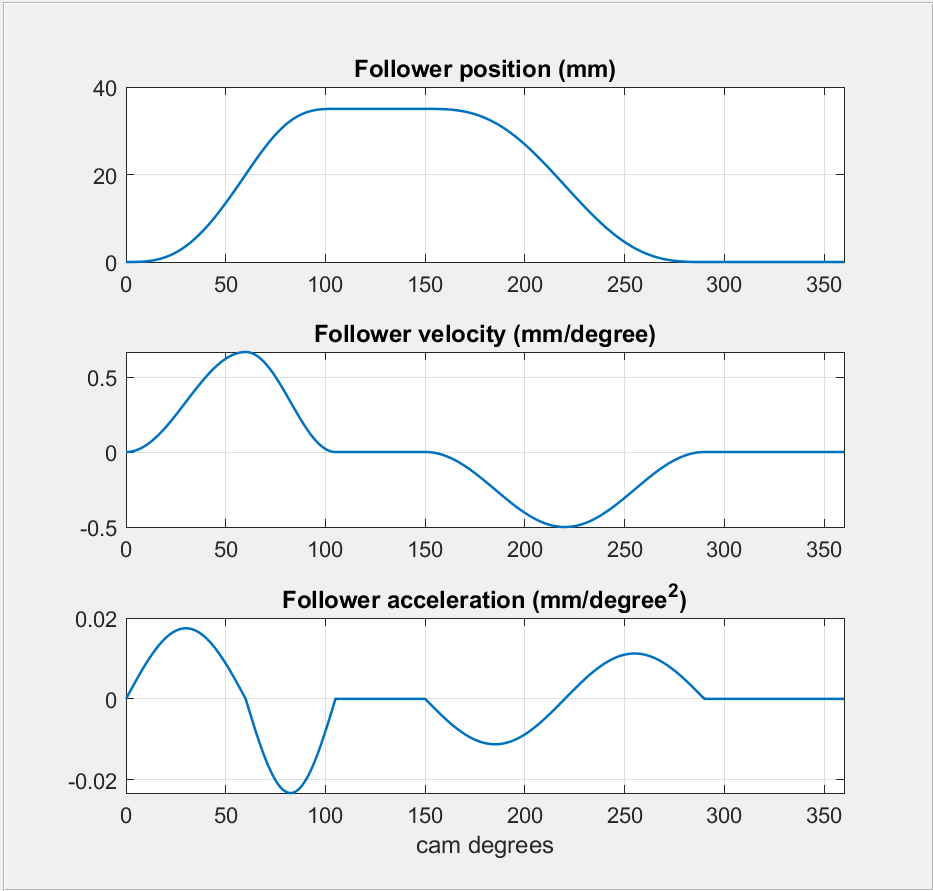
\includegraphics[width=.78\textwidth]{hefwet.png}
	\caption{The motion law \(S(\theta\) and its first and second derivatives in function of the cam angle \(\theta\). These plots were created with \texttt{matcam.m}}
	\label{fig:hefwet}
	
\end{figure}

The chosen segment sequence for this system consists of a C1, a C2 and a C6 segment and some dwells (segment with no rise or decline, which leads to a constant displacement).

\begin{itemize}

\item The first segment is a C1 half-cycloid which rises from 0 to +20 millimeters between 0 and 60 degrees. 

\item The second one is a C2 half-cycloid that rises from +20 to +35 millimeters between 60 and 105 degrees. By choosing to end this segment at 105 degrees, the first derivative of S is perfectly continuous in \(\theta=60°\).

\item After this second half-cycloid comes a dwell at +35 millimeters between 105 and 150 degrees. This dwell forms a perfectly continuous funtion with the C2 half-cycloid before it and the decreasing C6 cycloid behind it.

\item The last cycloidal part is a C6 segment that declines from +35 to 0 millimeters between 150 and 290 degrees.

\item To connect the C6 cycloid back with the C1 segment, a dwell at 0 millimeters is used between 290 and 360 degrees.

\end{itemize}

A graphical representation of this motion law and of its first and second derivatives is shown in figure~\ref{fig:hefwet}. On this plot one can see that the velocity is perfectly continuous and that the absolute value of the acceleration does not exceed 0,025~\(\si{mm/degree^2}\).




\section{Determining the geometry of the follower}
\label{sec:2}

\section{Verifying the rigid body forces}

\subsection{Sizing the spring}

\subsection{Instantaneous power}

The power to drive the cam is given for a non-excentric follower \cite{vermogen}:

\begin{equation}
	\begin{split}
	P(\theta) & = \vec{N}(\theta)\cdot\vec{v}(\theta) \\
	&=N(\theta)\cdot sin(\alpha)\cdot R(\theta)\cdot \omega
	\end{split}
\end{equation}

For the case where there is an excentrity \(e\neq0\), the power is calculated as follows:

\begin{equation}
	\begin{split}
	P(\theta) & = \vec{N}(\theta)\cdot\vec{v}(\theta) \\
	&=N(\theta)\cdot cos(\alpha)\cdot f'(\theta)\cdot\omega
	\end{split}
	\label{eq:verm_exc1}
\end{equation}

The pressure angle for a cam with an excentric follower is given in slide 31 of chapter 8 of the manual~\cite{cursus}: FIGUURFIGUURGIFURGIFURIFUFRIFUUUUUFFF

\begin{equation}
	\begin{split}
	\alpha& = arctan\left(\frac{f'(\theta)-e}{\sqrt{R_0^2-e^2}+f(\theta)}\right)\\
	&=arctan\left(\frac{f'(\theta)-e}{\sqrt{R(\theta)^2-e^2}}\right)
	\end{split}
	\label{eq:verm_exc2}
\end{equation}

And by using equation~\ref{eq:verm_exc2} in equation~\ref{eq:verm_exc1}, the power can be written as:

\begin{equation}
	\begin{split}
	P(\theta) =&~ N(\theta)\cdot cos(\alpha)\cdot \Big(tan(\alpha)\cdot\sqrt{R(\theta)^2-e^2}+e\Big)\cdot\omega\\
	=&~N(\theta)\cdot sin(\alpha)\cdot\sqrt{R(\theta)^2-e^2}\cdot\omega  +~N(\theta)\cdot cos(\alpha)\cdot e \cdot\omega
	\end{split}
\end{equation}

The power for both the case without excentricity and the case with excentricity (\(e=4,5~cm\) as determined in section~\ref{sec:2}) is calculated in the MATLAB function \texttt{power.m}. The plots of the powers in function of \(\theta\) can be found in figure~\ref{fig:powerplot}. Figure~\ref{diffpower} shows the difference between the two power plots. This difference is of an order of magnitude of \(10^{-14}\) and is due to the machine precision of MATLAB. The power for the cam with a centric follower is thus equal to the power for the cam with an excentric follower.

\begin{figure}
	\centering
	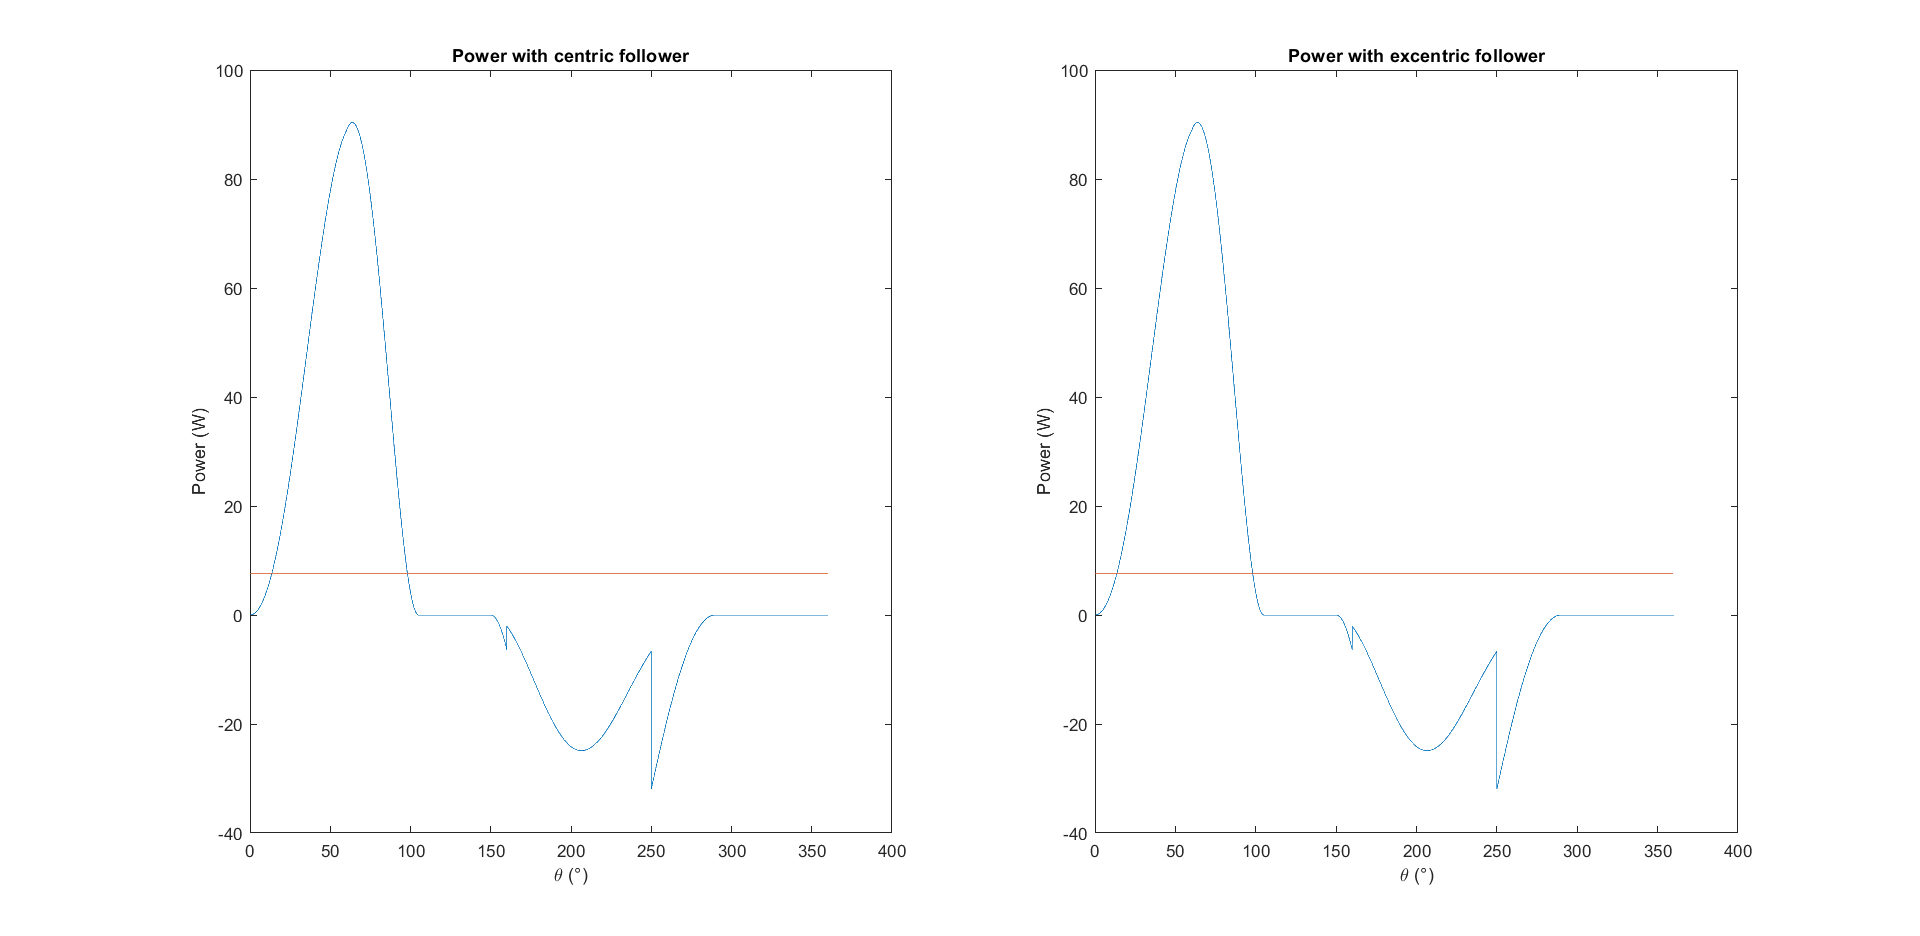
\includegraphics[width=\textwidth]{powerplot.png}
	\caption{The instantaneous power \(P\) to drive the cam in function of \(\theta\) for a centric and an excentric follower.}
	\label{fig:powerplot}
	
\end{figure}

\begin{figure}
	\centering
	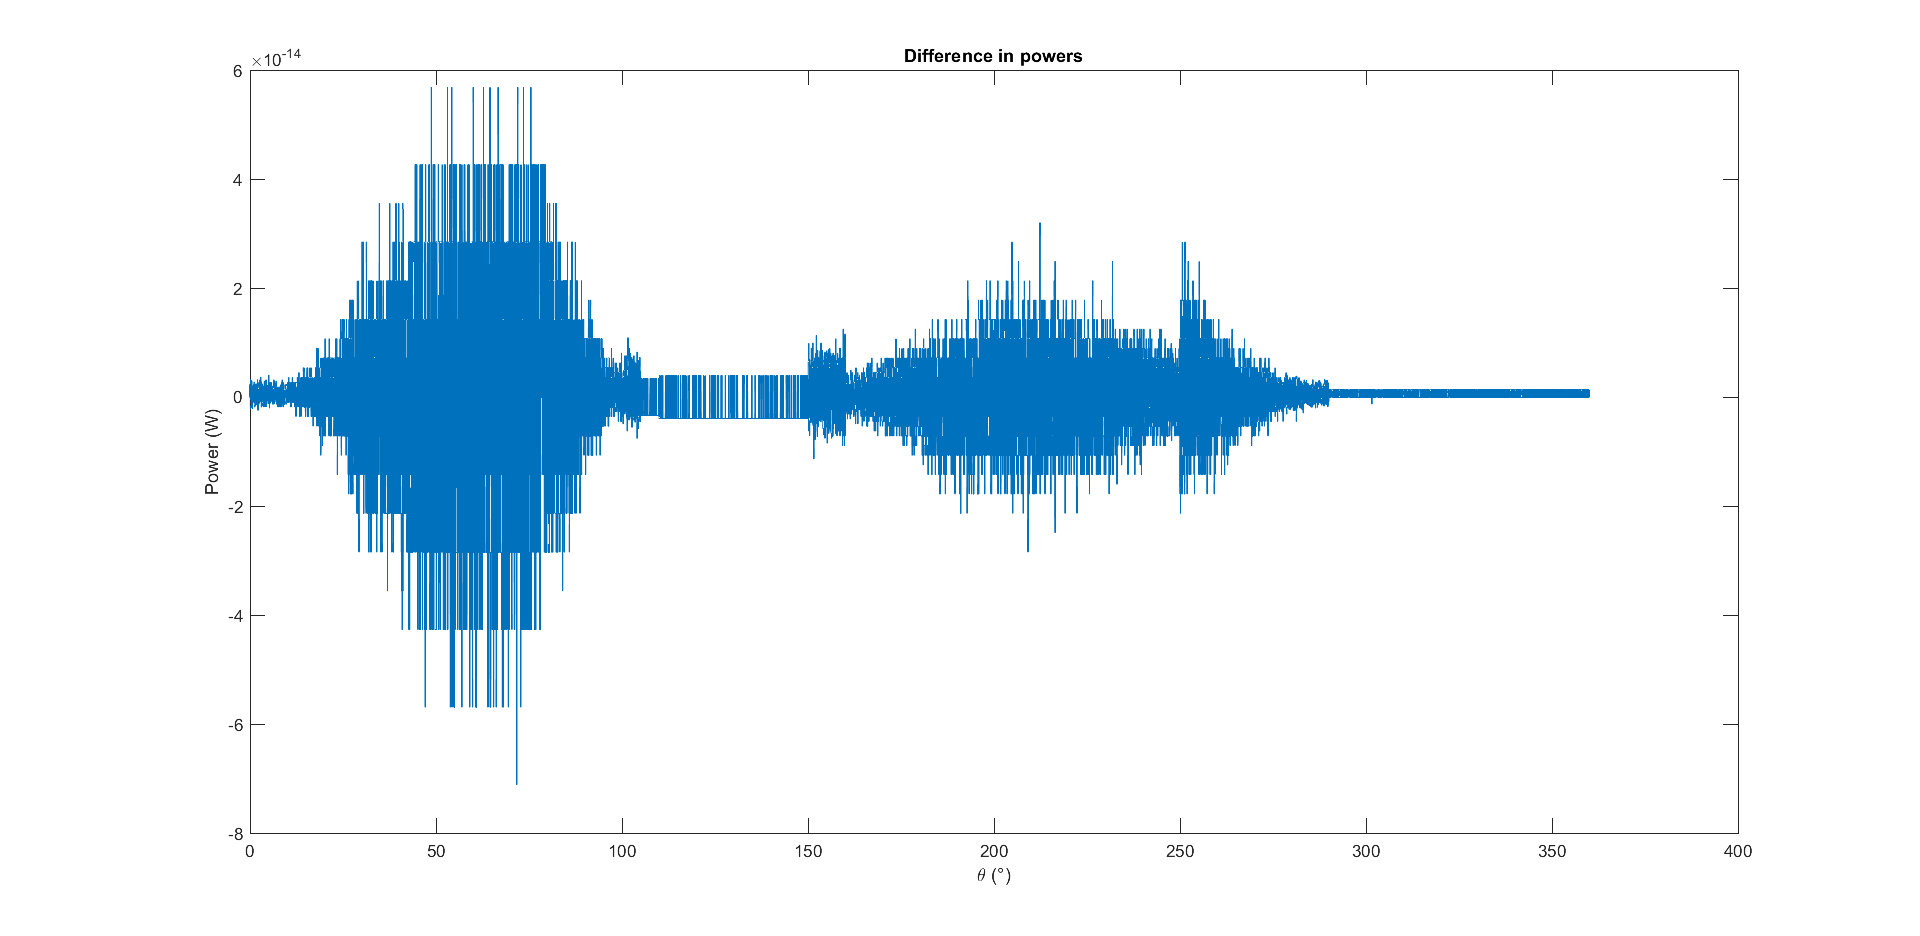
\includegraphics[width=\textwidth]{diffpower.png}
	\caption{Difference between the power with and without excentricity in function of \(\theta\).}
	\label{diffpower}
\end{figure}

\subsection{Designing a flywheel}

\section{Dynamics of the follower}

\bibliographystyle{plain}
\bibliography{nokken}

\end{document}